\section{Konzeption und prototypische Umsetzung}
In diesem Kapitel wird die prototypische Implementierung der Schnittstelle für die Anbindung von austauschbaren Datenquellen an KI-Algorithmen beschrieben. Zunächst werden die Anforderungen für das Projekt innerhalb der Bachelorarbeit erläutert. Anschließend wird das erarbeitete Konzept beschrieben. Dar mithilfe des Konzeptes entwickelte Prototyp sowie das anschließende Deployment findet sich ebenfalls in diesem Kapitel wieder.  

\subsection{Anforderungen}
Die Anforderungen für die Schnittstelle und den daraus resultierenden Prototypen wurden in Zusammenarbeit mit der CONET Solutions GmbH erhoben. Bei der CONET gab es ein offenes Forschung- und Entwicklungsprojekt zur Erstellung eines Trend-Scouting Systems. Das Ziel des Systems sollte es sein, eine Architektur bereitzustellen, die vom Nutzer gestellte Anfragen annimmt und diese mit einer KI analysiert, um Aussagen darüber treffen zu können, welche Technologien in der Zukunft relevant werden könnten. Da der Umfang eines Trend-Scouting Systems zu groß für den Zeitraum einer Bachelorarbeit ist, ergab sich als Zielsetzung die Entwicklung der Architektur, die ein solches System unterstützen könnte. Die genaue Anforderungserhebung wurde nach dem Leitfaden der von der \ac{iec} veröffentlichten Norm IEC 62304 Kapitel 5.2 entworfen.\footcite{daniel2018anforderungen} Innerhalb dieser Norm ist spezifiziert, wie Anforderungen an eine Software aufbereitet und dokumentiert werden sollen.

Im ersten Schritt wurden die Benutzerschnittstellen spezifiziert. Die grundlegende Interaktion mit dem System findet über die Website statt. Dort hat der Nutzer die Möglichkeit seine Suchanfrage in Form eines ausgeschriebenen Satzes oder über einzelne Stichpunkte in ein Textfeld einzugeben. Die nächste Benutzerschnittstelle ist die Transformation der zuvor eingegebenen Suchanfrage. Der Nutzer soll dort mittels JSON-Syntax die Suchanfrage modifizieren können. Dies ist im Hinblick auf eine eventuell automatisierte Nutzung des Systems erforderlich. Im dritten Schritt soll der Nutzer die Option haben, die Suchparameter für die KI anzupassen. Vor allem relevant ist die Anzahl der Ergebnisse, die bei einer gestellten Suchanfrage zurückgegeben werden. An dieser Stelle soll aber auch weitere Parameter eingegeben werden können. Anschließend ist eine Möglichkeit vorgesehen die Anfrage inklusive der Parameter abzuschicken. In Abbildung 5 ist die Interaktion mit dem System in einem Use Case Diagramm dargestellt.

\begin{figure}[H]
  \centering
    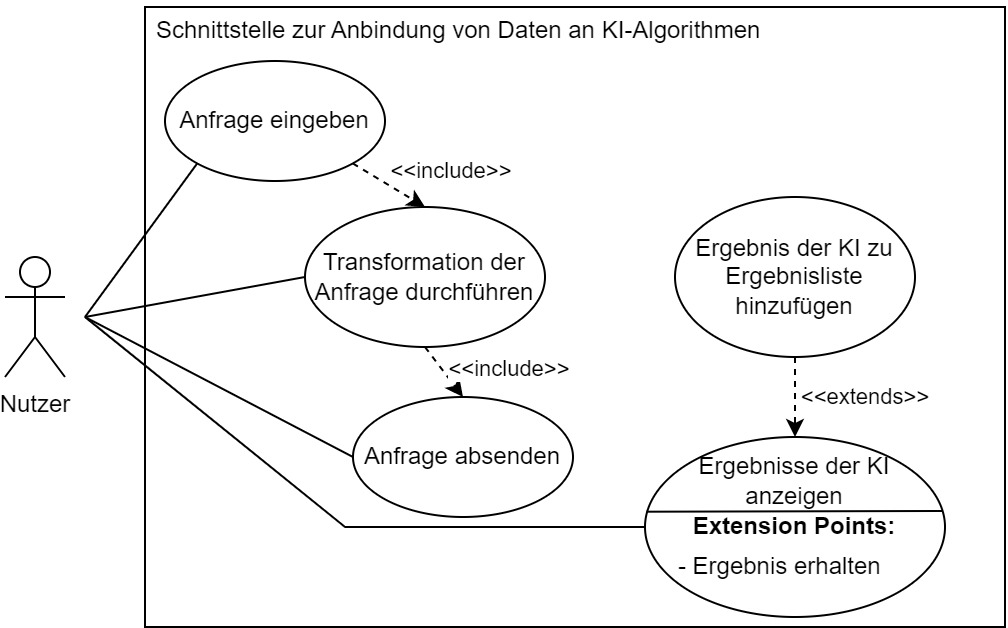
\includegraphics[width = 15cm]{bilder/UseCase}
    \caption{Use Case Diagramm der Interaktion mit der Schnittstelle}
\end{figure}

Die letzte Möglichkeit, die der Nutzer hat, mit der Schnittstelle zu interagieren, ist über die API selbst. Dort gibt es eine Route, über die die aktiven KI-Services verwaltet werden können. Abhängig von der gewählten HTTP-Methode sollen verschiedene Funktionen angeboten werden. Die drei Hauptfunktionen sind die Auflistung aller aktiven Services, das erstellen eines neuen Services und das löschen eines Services.

Der nächste Schritt der Anforderungsanalyse nach IEC 62304 ist die Festlegung des \ac{gui}. Die grafische Oberfläche sollte sich auf eine Seite beschränken und in drei Bereiche eingeteilt sein. Jeder der Bereiche beinhaltet eine Kachel mit einer Überschrift. Die drei Überschriften \glqq Query\grqq{}, \glqq Transformation\grqq{} und \glqq Service\grqq{} sollen verdeutlichen, welche Aktionen in der entsprechenden Kachel passieren.
Der linke Bereich der Seite für die Query beinhaltet die Eingabe durch den Nutzer, welche durch ein Textfeld realisiert wird. Des Weiteren gibt es einen Button zum Hochladen der Anfrage an den Server. Im mittleren Bereich der Seite befindet sich die Kachel für die Transformation der Eingabe. Der Inhalt der Kachel selber ist nochmal in drei Bereiche aufgeteilt. Der erste Bereich zeigt die vom Nutzer hochgeladene Eingabe. In diesem Feld kann der Nutzer keine Änderungen vornehmen. Das zweite Feld enthält die Eingabe für die Transformation. Das Textfeld enthält einen vorgefertigter Text in JSON-Syntax, den der Nutzer anpassen kann. Unter dem Textfeld gibt es einen Button, der die Funktion hat, die Transformationsanleitung an den Server zu senden. Im dritten Feld wird das Ergebnis der Transformation angezeigt, damit der Nutzer überprüfen kann, ob das erzeugte Ergebnis seinen Erwartungen entspricht. 
Der rechte Bereich der Seite ist für die Auswahl und Nutzung der KI-Services vorgesehen. Der gewünschte Service soll über ein Dropdown ausgewählt werden. Da die Services für ihre Anfragen Parameter übergeben bekommen müssen, muss eine Tabellenstruktur implementiert werden. Die Tabelle hat zwei Spalten und beliebig viele Reihen. Innerhalb der Tabelle können Schlüssel-Wert Paare eingegeben werden, wobei der Schlüssel in der ersten Spalte und der Wert in der zweiten Spalte steht. Unter der Tabelle muss es einen Button geben, der die Anfrage an den KI-Service sendet. Daraufhin startet der Abfrageprozess der die Antworten der KI-Services zusammenträgt. Die Ergebnisse des KI-Services werden in einem Feld unter dem Button angezeigt. Bei jedem Ergebnis wird zunächst nur die Überschrift angezeigt. Erst bei einem Klick auf die Überschrift soll der Inhalt ausgeklappt werden.

Der Schritt nach der Anforderungserhebung der grafischen Oberfläche ist die Dokumentation des Verhaltens des Systems. Besonderer Fokus liegt hierbei auf dem Verhalten gegenüber Nutzerinterkationen. Beim ersten Bescuh der Website, wird dem Nutzer ein Token zugesendet, welche für alle weitere Anfragen zur Authentifizierung an der API genutzt werden soll. Innerhalb des Tokens ist eine eindeutige User ID hinterlegt. Nachdem der Nutzer auf der linken Seite der Website in der Kachel \glqq Query\grqq{} den Upload Button gedrückt hat, sendet die Website den eingegebenen Text an die API. Dabei soll im Authorization Header der Token stehen und im Request Body der eingegebene Text in JSON-Syntax. Ist die Anfrage beim Server eingegangen, soll sie in einem Redis Cache hinterlegt werden und anschließend wieder ans Frontend zur Bestätigung zurückgesendet werden. Sollte bei der Anfrage ein Fehler aufgetreten sein, wird der Statuscode 500 an die Website zurückgegeben und das Ergebnis des Uploads wird nicht im ersten Feld der Transformation angezeigt. Sollte der Upload erfolgreich gewesen sein, wird der Text dort angezeigt und der Nutzer hat die Möglichkeit, eine Transformationsanleitung in JSON-Syntax einzugeben und diese über den \glqq Transform\grqq{} Button an das Backend zur Auswertung zu schicken.

%\subsubsection{Benutzerschnittstellen}

%\subsubsection{GUI}

%\subsubsection{Verhalten des Systems}

%\subsubsection{Geschwindigkeit des Systems}

%\subsubsection{Umgebung und Installation}

%\subsubsection{Benutzerfehler und Überlast}
%- Benutzerschnittstelle(n)
%- Die GUI: Positionierung von Elementen, Style Guides, …
%- Verhalten des Systems auf Benutzeraktionen im Normal- und Fehlerfall: Vom System angezeigte Informationen, Berechnungen, Grafiken, Meldungen, Warnungen, “Screenflow”, …
%- Die Geschwindigkeit, mit der diese Reaktionen geschehen
%- Auf welchen Umgebungen, sich die Software (Blackbox) installieren lassen soll (Betriebssystem, vorausgesetzte Datenbanken und andere Server, Hardware einschließlich RAM) und wie diese Installation von statten gehen soll.
%- Wie sich das System auf Benutzerfehler und Überlast reagieren soll.
%
%- modularisierung der einzelnen bereiche
%- trennung von front und backend
%- implementierung eines ki-services, der text in vektoren konvertiert
%- vektor zur textähnlichkeitssuche in elasticsearch
%- skalierbarkeit der ki-services
%- webbasierte implementierung
%- (performante auswertung der anfragen)
%- api mit rest implementiert
%- absturzsicherheit
%- logging von events
%- deployment über docker

\subsection{Konzeption}


% 4 Sichten Modell von Starke
% Kontextsicht, Laufzeitsicht, Bausteinsicht, Verteilungssicht

\subsubsection{Softwarearchitektur}
%Mehr Diagramme - Use Case UML zu Abbildung auf Klassen
Ein grundlegender Dienst, der Daten mit einer KI verbindet, kann mithilfe eines einzigen Python-Scripts erstellt werden. Die Herausforderung an einer praxistauglichen Anwendung, die gleichzeitig von mehreren Usern genutzt werden kann, liegt im  Architekturdesign der Software. Eine praxistaugliche Anwendung muss neben den funktionalen Anforderungen auch noch weitere nicht funktionale Anforderungen erfüllen. Die drei wichtigsten nicht funktionalen Anforderungen sind Performance, Skalierbarkeit und Verfügbarkeit. Alle drei Anforderungen können mit einem lokal ausgeführten Skript nicht erfüllt werden. 

Damit Nutzer mit der Software interagieren können, wird ein Frontend benötigt. Ein zentral gehostetes, webbasiertes Frontend kann von einem Nutzer über eine einfache URL im Webbrowser aufgerufen werden. Für die anzuzeigenden Daten im Frontend wird eine Verbindung zum Backend benötigt. Diese wird über eine HTTP Verbindung zur mit Flask gehosteten REST API bereitgestellt.

Um die Anforderung der Skalierbarkeit erfüllen zu können, ist die REST-API komplett zustandslos implementiert worden. Eine API ohne Zustände speichert keine Zwischenstände zu den Anfragen einzelner Nutzer. Bei jeder Anfrage an die API müssen alle Informationen im Request bereitgestellt werden, die die API zum bearbeiten der Anfrage benötigt. Dies bietet die Möglichkeit bei steigender Nutzerzahl mehrere parallel betriebene Instanzen der API hochzufahren. Dadurch ist eine horizontale Skalierung gewährleistet. Horizontal skalierbare Instanzen innerhalb der Software Architektur sind in Abbildung 1 mit zwei hintereinander gestapelten Rechtecken visualisiert.

Da die Kommunikation zwischen dem Frontend, der API und den KI-Services asynchron läuft, muss das Flask Backend trotz seiner Zustandslosigkeit Transformationsanleitungen und Ergebnisse der KI-Services zwischenspeichern, bis sie im Frontend benötigt werden. Um die Performanceanforderungen erfüllen zu können, können nicht alle Zwischenstände in einer MySQL Datenbank gespeichert werden. Die Lese- und Schreibgeschwindigkeit kann bei steigender Nutzerzahl problematisch werden. Um dem Entgegenzuwirken wird ein Redis Key-Value Store als Cache betrieben. Die zwischengespeicherten Daten werden nach dem ersten Aufruf wieder gelöscht, weswegen eine persistente Speicherung nicht notwendig ist. In-Memory Datenbanken speichern und führen ihre Queries direkt im RAM aus, wodurch Anfragen im Vergleich zu einer MySQL Datenbank deutlich schneller ausgeführt werden.

Im Flask Backend werden alle Routen und die meisten Funktionen abgekapselt in einem Funktion Wrapper ausgeführt. Dieser fungiert als eine Art Sandbox, in der auftretende Fehler nicht zum Programmabsturz führen, sondern behandelt und geloggt werden können. Alle Logs werden persistent in einer MySQL Datenbank gespeichert. Mit dem Dienst Grafana können diese Logs angezeigt werden.

Die Laufzeit von KI-Services kann sehr stark vom verwendeten KI-Modell, der zu durchsuchenden Datenmenge, wie auch der vom Nutzer gesendeten Eingabe abhängen. Bei einer synchronen Kommunikation zwischen dem Flask Backend und dem Service können sehr lange Wartezeiten entstehen. Wenn der KI-Service ebenfalls eine REST-Schnittstelle implementieren würde, könnten es bei einem HTTP Request zum Timeout der Anfrage führen. Aufgrund der schwanken Laufzeit muss eine asynchrone Kommunikationsstruktur, wie RabbitMQ mit dem AMQP implementiert werden.

Die einzelnen Services können mit einem Eintrag in der MySQL Datenbank registriert werden. Für die Registrierung muss lediglich der Name und der im Frontend anzuzeigende Name des Services hinterlegt werden. Die Registrierung eines Dienstes kann durch den Aufruf einer Route in der API durchgeführt werden. 

Der im Prototypen implementierte KI-Service nutzt das BERT Modell von Google zum konvertieren der Nutzereingaben in semantische Vektoren. Es wird ebenfalls eine Elasticsearch Datenbank betrieben, in der alle zu Durchsuchenden Einträge gespeichert sind. Im Gegensatz zu einer MySQL Datenbank, kann in einer Elasticsearch Datenbank zu jedem Eintrag ein semantischer Vektor gespeichert werden. Der KI-Service kann mithilfe der Kosinusähnlichkeitssuche den semantischen Vektor der Eingabe mit den Vektoren der Datenbank vergleichen und so die semantisch ähnlichstes Texte herausfiltern. Die gefunden Einträge werden über RabbitMQ im Anschluss wieder an das Flask Backend geschickt, damit sie dort vom Frontend ausgelesen werden können.

\begin{figure}[H]
  \centering
    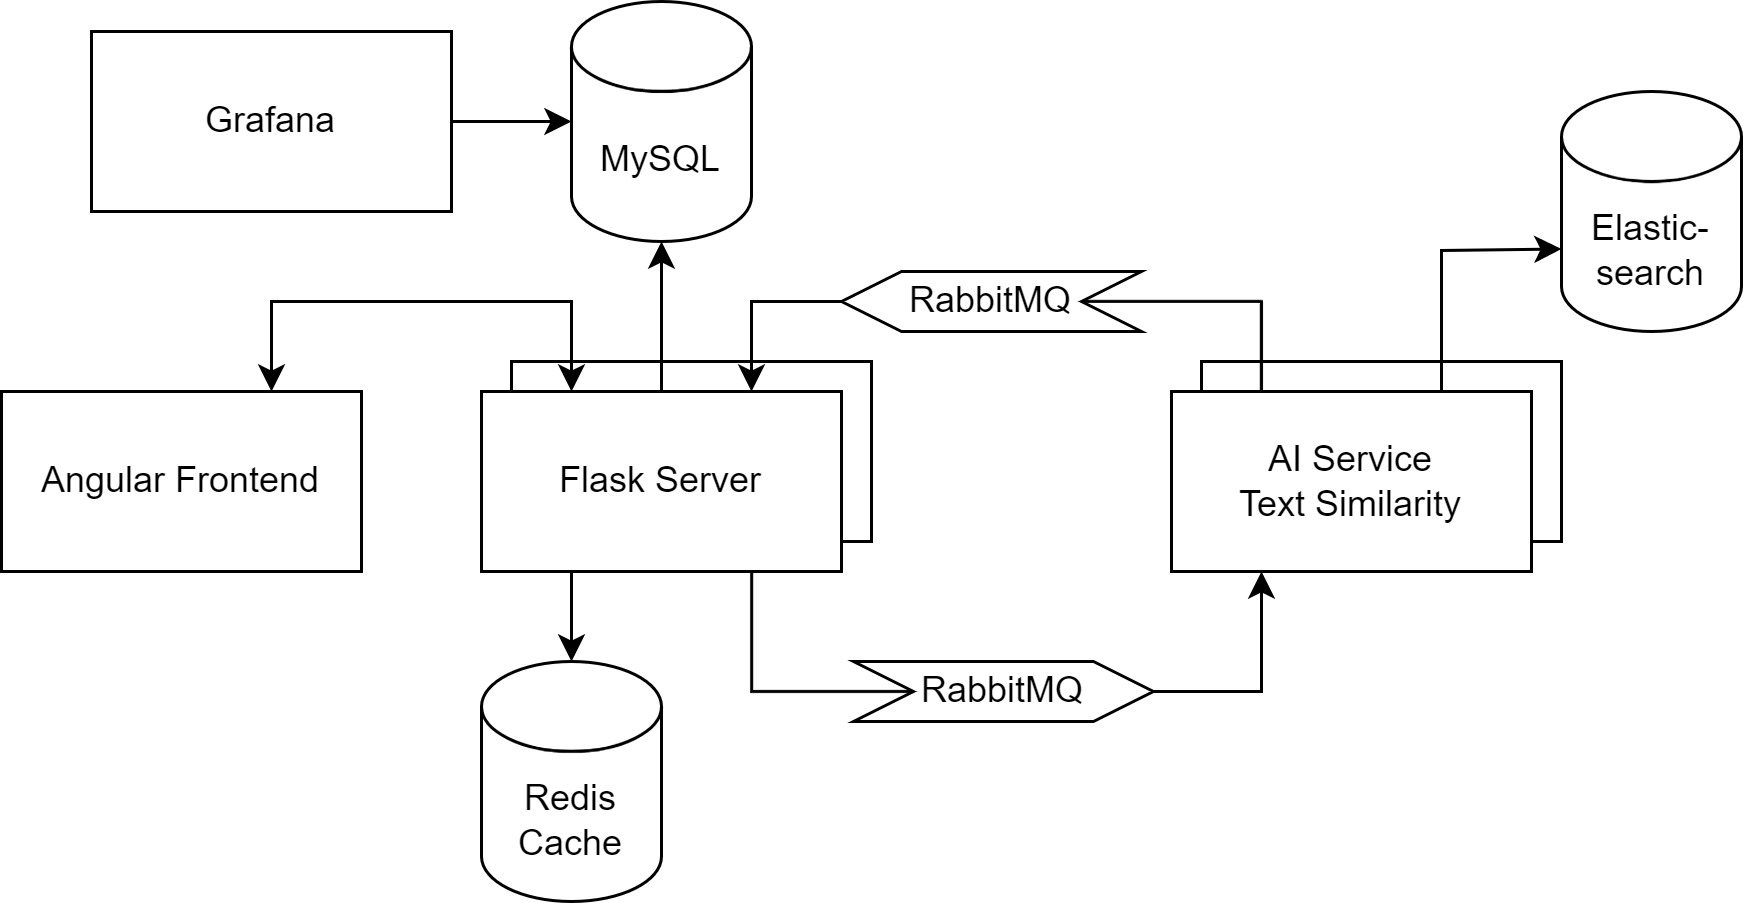
\includegraphics[width = 15cm]{bilder/Architektur}
    \caption{Softwarearchitekturdiagramm}
\end{figure}

\subsubsection{Programmablauf}
text
\subsubsection{KI-Services}
text 
\subsection{Prototypische Umsetzung}
text
\subsubsection{Implementierung der REST-API}
Python bietet mit dem Package Flask die Möglichkeit einen simplen und gut skalierbaren Webserver aufzusetzen. Für das Starten einer Flask Instanz muss das Package Flask in die Python Umgebung importiert werden. Anschließend kann ein Flask-Objekt erzeugt und die Flask Instanz mit den gewünschten Parametern gestartet werden.

\begin{lstlisting}[language=Python]
from flask import Flask
app = Flask(__name__)
app.run(host="0.0.0.0", port=80, use_reloader=False)
\end{lstlisting}

Damit die API auch automatisiert aus einem Docker Container heraus gestartet werden kann, muss die Ausführung des Flask Services in die Main Methode von Python ausgelagert werden. Flask blockiert den Thread auf dem es ausgeführt wird, was eine asynchrone Kommunikation über RabbitMQ nicht möglich macht. Der Receiver benötigt seinen eigenen Thread, weswegen eine Multithreading-Architektur implementiert werden muss. Zu diesem Zweck wird das threading Package genutzt. Über den Parameter \texttt{daemon} kann bei der Erzeugung eines Threads festgelegt werden, dass der Thread im Hintergrund läuft und den Hauptthread nicht blockiert.

\begin{lstlisting}[language=Python]
def start_server():
    app.run(host="0.0.0.0", port=80, use_reloader=False)

if __name__ == '__main__':
    thread_server = threading.Thread(target=start_server, daemon=True).start()
\end{lstlisting}

Eine in der API adressierbare Route kann in Flask über Function-Annotations definiert werden. Die von Flask implementierten Anntotations haben die Form \texttt{instanz.route('path', methods=["METHOD"])}. Der Name der Instanz wird am Anfang des Projekts als \texttt{app} definiert. Der \texttt{path} beschreibt die Route, die vom Frontend aufgerufen werden muss, damit die nachfolgende Funktion ausgeführt wird. Im Array \texttt{methods} besteht die Möglichkeit, ein oder mehrere Request Typen zu definieren, die die Funktion akzeptieren soll.

Eine beispielhafte Nutzung der Annotations, um eine Route in der API zu definieren, ist nachfolgend aufgeführt. 

\begin{lstlisting}[language=Python]
@app.route('/', methods=["GET"])
def index():
    [..]
    return r.respond({"token": token}, cookie=f"Authorization={token}")
\end{lstlisting}

Der Inhalt der Methode und deren genaue Funktionsweise wird in den folgenden Kapiteln näher erläutert.

Die Funktion \texttt{respond} ist im Skript \texttt{api/response\_{}generator.py} definiert. Sie dient als Function Wrapper, der bei jeder ausgehenden Response die Response-Header, eventuelle Cookies und den Reponse Typen setzt. Der Output der Response wird mithilfe des \texttt{json} Packages in JSON Syntax konvertiert.

\begin{lstlisting}[language=Python]
import json
from flask import Response
def respond(r, status=200, json_dump=True, cookie=""):
    [...]
    return Response(json.dumps(r), status=status, mimetype='application/json', headers=headers)
\end{lstlisting}

In Tabelle 1 sind alle in der API verfügbaren Routen aufgelistet. Auf die genaue Funktionalität der einzelnen Funktionen wird in den folgenden Kapitel eingegangen.

\begin{table}[H]
\centering
\begin{tabular}{c|c|l}
\textbf{Route} & \textbf{Typ} & \textbf{Funktion}\\
\hline
\texttt{'/'} & \texttt{GET} & Erstellung eines JSON Web Tokens\\
\hline
\texttt{'/upload/file'}  & \texttt{POST} & Hochladen einer Textdatei für den Input der KI \\
\texttt{'/upload/text'}  & \texttt{POST} & Texteingabe für den Input des KI-Services \\    
\texttt{'/transform'}  & \texttt{POST} & Festlegen der Tranformationseigenschaften\\ 
\texttt{'/send'}  & \texttt{POST} & Transformieren und Senden des Inputs an einen KI-Service \\ 
\texttt{'/poll'}  & \texttt{GET} & Abfrage der vom KI-Service gelieferten Ergebnisse \\ 
\hline
\texttt{'/service'}  & \texttt{GET} & Auflistung aller Services \\
\texttt{'/service'}  & \texttt{POST} & Registrieren eines neuen Services \\ 
\texttt{'/service'}  & \texttt{DELETE} & Löschen eines Services \\       
\end{tabular}
\caption{Implementierte Routen der REST-API}
\end{table}

\subsubsection{Nutzeridentifizierung mit JWT}
Innerhalb des Backendes ist es notwendig, einzelne Nutzer voneinander zu unterscheiden. Für jeden Nutzer speichert das Backend den hochgeladenen Text, die Transformationsanleitung und die Antworten des angefragten KI-Services im Redis Cache. Um Nutzer voneinander unterscheiden zu können, gibt es zwei grundlegende Möglichkeiten. 
\begin{enumerate}
\item Identifizierung durch den Nutzer der Software. Beispielsweise mittels Registrierung durch E-Mail Adresse und Passwort.
\item Identifizierung durch das Backendend der Software. Generierung und Zuweisung einer zufälligen aber eindeutigen User-ID.
\end{enumerate}

Die Erhebung von personenbezogenen Daten setzt die Einhaltung der \ac{dsgvo} voraus. Dies bedeutet einen erheblichen Mehraufwand für eine Anwendung, die sonst keinen weiteren Nutzen aus den Daten zieht.

Das Backend nutzt einen \ac{uuid} der sich durch das Python Package \texttt{uuid} generieren lässt. Eine UUID ist eine 32 Zeichen lange Zahl im Hexadezimalformat. Die importierte Funktion \texttt{uuid4()} erzeugt eine zufällige, ohne von Parametern beeinflusste UUID. Der Nutzer muss diese UUID mitgeteilt bekommen und für alle seine Anfragen, aufgrund der zustandslosen Implementierung der API, im Authorization Header mitschicken. Damit die UUID nicht ausgelesen oder manipuliert werden kann, wird sie nicht als einfacher Text in der Response an den Nutzer geschickt, sondern vorher in ein JSON Token geschrieben und verschlüsselt.

Ein \ac{jwt} ist ein kompaktes, URL-sicheres Mittel zur Darstellung von Forderungen, die zwischen zwei Parteien übertragen werden sollen. Die Angaben in einem JWT werden als JSON-Objekt kodiert. Der Inhalt des JST kann digital signiert oder die Integrität mit einem \ac{mac} geschützt und/oder verschlüsselt werden.\footcite{jones2015json}

Im nachfolgenden Codeausschnitt ist die Generierung der UUID und die Verschlüsselung des JWT dargestellt.
\begin{lstlisting}[language=Python]
def uuid_gen():
    return uuid.uuid4()
    
def encode_token(param):
    return jwt.encode(param, JWT_PASSWORD, algorithm="HS256")

token = encode_token({'uid': str(uuid_gen())})
\end{lstlisting}

Für jede Route, ausgenommen die \texttt{/service} Routen zum Management der Services, wird der JWT für die Ausführung benötigt. Die Überprüfung und Entschlüsselung des Tokens ist für jede Route gleich, daher ist es sinnvoll diese Funktionalität zu zentralisieren. Damit wird die Fehleranfälligkeit reduziert und und die Wartbarkeit erhöht, sollte sich zum Beispiel der Algorithmus oder das Passwort für die Verschlüsselung ändern. Wie auch Flask Annotations zum definieren einer Route verwendet, ist es möglich eigene Annotations zu entwerfen. Für diese Funktion ist das Python Package \texttt{functools} mit der Funktion \texttt{wraps} zuständig. Wraps ermöglicht es, Funktionen ineinander zu verschachteln.

Im Prototypen wird die Funktion \texttt{token\_{}required(f)} definiert. Diese Funktion dient als eine Umgebung, in der eine weitere Funktion ausgeführt werden. Im Gegensatz zur normalen Ausführung einer Funktion, werden in der \texttt{token\_{}required(f)} Funktion vor der Ausführung der eigentlichen Funktion mehrere Rahmenbedingungen geprüft. Der vom Nutzer gesendete Token muss nach der erfolgreicher Entschlüsselung syntaktisch korrektes JSON enthalten. Sollte dies nicht der Fall sein, wird die die eigentliche Funktion, die zur API Route gehört, gar nicht erst ausgeführt. Der Nutzer bekommt direkt eine Response mit dem HTTP Error-Code 401: Unauthorized gesendet. \footcite{fielding1999rfc2616}

Wenn die Entschlüsselung des Tokens erfolgreich war, wird die innere Funktion ausgeführt. Als Parameter der inneren Funktion wird die im JWT enthaltene UUID übergeben. Durch diesen Aufbau ist der Code für die Verifizierung des Tokens und die Logik der Funktion unter der angesprochenen Route vollständig getrennt.

\begin{lstlisting}[language=Python]
@routes.route('/upload/text', methods=['POST'])
@token_required
def upload_text(uid):
    [...]
\end{lstlisting}

\subsubsection{Caching mit Redis Datenbank}
Redis ist ein Key-Value Store der vollständig im RAM ausgeführt wird. Innerhalb von Redis sind mehrere Datenbanken definiert, die in ihrer Standartkonfiguration über einen Index $i$, mit $0\leq{}i<16$ aufgerufen werden. Im Backend werden die ersten drei Datenbanken verwendet.
\begin{enumerate}
 \item Datenbank 0: Cache der hochgeladenen Textdateien für den Input der KI
 \item Datenbank 1: Cache der Transformationsanleitung
 \item Datenbank 2: Cache der vom KI-Service produzierten Ergebnisse
\end{enumerate} 

\subsubsection{Kommunikation zwischen Backend und Services mit RabbitMQ}
Für den Informationsaustausch zwischen dem Backend und den verschiedenen KI-Services ist eine asynchrone Kommunikation implementiert. Je nach Komplexität des Services, kann die Verarbeitung einer vom Nutzer gestellten Anfrage mehrere Sekunden bis Minuten dauern. Eine synchrone Kommunikation, in der der Client auf unbestimmte Zeit auf eine Antwort wartet ist nicht möglich. Wenn nach einer vom Browser definierten Zeit keine Antwort auf den Request kommt, wird der Request mit einem Timeout abgebrochen. Sollte die KI nach der maximal verfügbaren Zeit ihr Ergebnis liefern, wird dieses Verworfen und ner Nutzer muss eine neue Anfrage stellen. Damit Anfragen nicht verloren gehen und die Antworten dem Server mitgeteilt werden können, wenn sie bereit sind, wird der Message Broker RabbitMQ implementiert. 

RabbitMQ dient als Middleware, die Anfragen vom Server annimmt und diese im in einer Queue zwischenspeichert, um sie anschließend an die Services zu verteilen. Damit die Nachrichten in eine Queue geschrieben werden können, muss im ersten Schritt eine Verbindung zu RabbitMQ aufgebaut werden. Mithilfe des Packages \texttt{pika} kann über den Host, unter dem RabbitMQ erreichbar ist, den Port 5672 und den Login-Credentials eine TCP Verbindung aufgebaut werden.

Innerhalb einer Connection, können über einen Channel können sowohl der Server, als auch die Services eine Verbindung mit dem RabbitMQ Dient aufbauen. Ein Channel beschreibt die logische Verbindung zwischen dem Server/Service und dem Broker. Für jede TCP Verbindung mit RabbitMQ können mehrere Channels erstellt werden.\footcite{dossot2014rabbitmq}

In einem Channel wird letztendlich die Queue definiert, in der die Nachrichten zwischengespeichert werden. Im folgenden Codeausschnitt ist gezeigt, wie eine Connection, ein Channel und eine Queue erstellt werden.

\begin{lstlisting}[language=Python]
def produce(uid, service, query, params):
    connection = pika.BlockingConnection(pika.ConnectionParameters(rabbit_host, 5672, '/', credentials))
    channel = connection.channel()
    channel.queue_declare(queue=service)
\end{lstlisting}

Die Nachrichten, die der Server an die Services schickt, werden mittels der im Channel definierten Methode \texttt{basic\_{}publish} in die für den Service entsprechende Queue geschrieben werden. Im vorherigen Codeausschnitt wird der Parameter \texttt{service} in der \texttt{produce} Methode übergeben. Dieser ist abhängig vom Service, an den die Anfrage gerichtet ist. Im Prototypen wurde der Service \texttt{text-similarity} implementiert. Dieser kann im Frontend als Ziel ausgewählt werden. Wenn der Nutzer im Frontend die Anfrage an den \texttt{text-similarity} Service stellt, wird die Methode \texttt{produce} mit dem String \texttt{\glqq text-similarity\grqq{}} aufgerufen.

Sollte es die Queue mit dem aufgerufenen Service noch nicht geben, wird diese von RabbitMQ beim ersten Aufrufen erstellt. Ist sie bereits vorhanden, wird lediglich ein Eintrag in die entsprechende Queue geschrieben.

Die Nachricht, welche aus der Anfrage des Nutzers, den eingegebenen Parametern und weiteren im Backend automatisch generierten Parametern, wie dem UUID, besteht, wird anschließend mittels AMQP an den Rabbit Broker gesendet. Dort wird die Nachricht, wie zuvor beschrieben, in die entsprechende Queue eingetragen. 

Auf Seiten des Services wird eine Methode implementiert, die die Nachrichten in einer Queue auslesen kann. Zu beginn muss eine Queue definiert werden, aus der Nachrichten ausgelesen werden. Dies funktioniert analog zum erstellen einer Queue für das Schreiben von Nachrichten über \texttt{queue\_{}declare} gefolgt von dem Namen der Queue. Das Registrieren als Consumer für eine Queue wird mittels der Methode \texttt{basic\_{}consume()} durchgeführt. Innerhalb der Parameter ist eine Callback Methode definiert, die ausgelöst wird, wenn der Service eine Nachricht erfolgreich aus der Queue ausgelesen hat. Die \texttt{callback} Methode ist der Startpunkt des Services, von dem aus die eingehende Nachricht mithilfe der KI analysiert und verarbeitet wird.

Um den Consumer zu starten und damit auf neue Nachrichten in der Queue zu warten, wird die Methode \texttt{start\_{}consuming()} ausgeführt. Im nachfolgenden Codesegment ist der eben beschriebene Prozess im KI-Service aufgeführt.

\begin{lstlisting}[language=Python]
channel.queue_declare(queue='text-similarity')
channel.basic_consume(queue='text-similarity',
                          auto_ack=True,
                          on_message_callback=callback)
channel.start_consuming()
\end{lstlisting}

Nachdem die KI die eingehende Anfrage verarbeitet hat, schreibt der Service die Response in eine Queue. Es kann jedoch nicht die gleiche Queue für Anfragen und Antworten verwendet werden, da es sonst dazu führen könnte, dass vom Service produzierte Antworten wieder als Anfrage interpretiert werden und es so zur fehlerhaften Ausführung des KI-Algorithmus kommt. Ein weiteres Problem wäre, dass die Antworten dann aus der Queue herausgenommen wurden und der Server keine Antwort mehr zur gestellten Anfrage erhält. Um dem entgegenzuwirken wurde eine zweite \glqq Response-Queue\grqq{} implementiert, in die ausschließlich die Antworten des Services geschrieben werden. Da die Queues über ihren Namen definiert werden, hat jede Response Queue einen vom Service abhängigen, automatisch generierten Namen. Der Name hat die Form \texttt{response-\{service\}}. Im Falle des \texttt{text-similarity} Services, hat die Antwort Queue den Namen \texttt{response-text-similarity}. 

\begin{lstlisting}[language=Python]
channel.queue_declare(queue='response-text-similarity')
channel.basic_publish([...], body=f'{{"uid": "{uid}", "service": "{service}", "message": {json.dumps(message)}}}'.encode('utf-8'))
\end{lstlisting}

Der Server implementiert, ähnlich wie der Service auch, eine Möglichkeit die Nachrichten in der Response Queue auszulesen. Innerhalb der Nachricht, die an den Service geht und vom Service wieder zurück kommt, wird die UUID des Nutzers mitgeliefert. Damit ist eine anschließende Zuordnung von Anfrage und Antwort möglich. Das Backend speichert die Antwort des KI-Services im Redis Cache und kann sie dem Frontend bei Bedarf zur Verfügung stellen.

Der Ablauf der Kommunikation zwischen dem Server und den Services mit RabbitMQ ist in Abbildung 4 veranschaulicht. 
\begin{figure}[H]
  \centering
    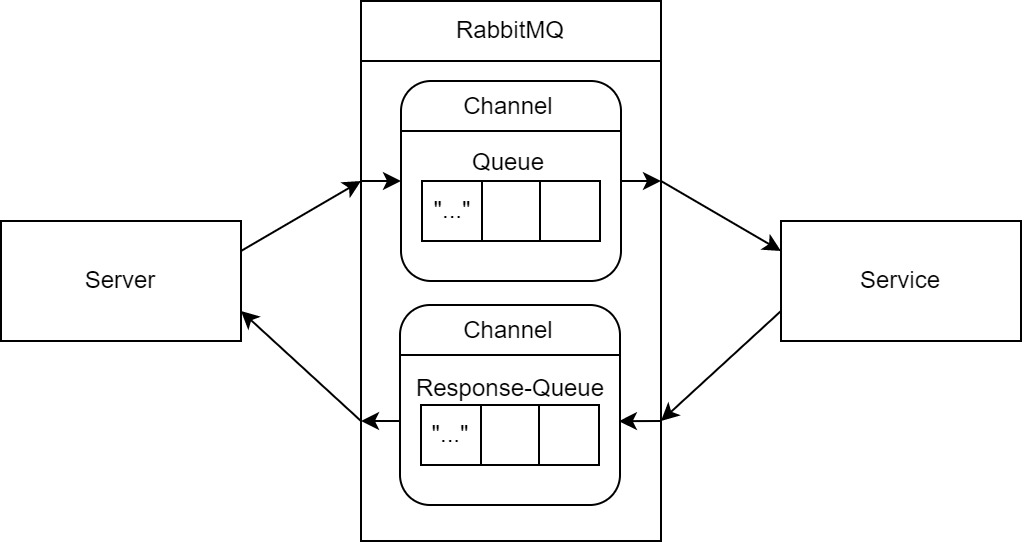
\includegraphics[width = 15cm]{bilder/Rabbit3}
    \caption{Kommunikation mit RabbitMQ}
\end{figure}

\subsubsection{Implementierung des KI-Services}
Der implementierte KI-Service lädt im ersten Schritt das KI-Modell, um mit diesem für jeden Eintrag in der Elasticsearch Datenbank einen semantischen Vektor zu generieren. Dieser semantische Vektor wird ebenfalls in der Datenbank gespeichert und kann für zukünftige abfragen genutzt werden.
Nachdem alle Einträge in der Elasticsearch Datenbank indiziert wurden, beginnt die Programmablaufschleife. Der erste Schritt der Schleife ist das warten auf eingehende Nachrichten. Diese Nachrichten werden über RabbitMQ aus der, für den Service definierten, Queue ausgelesen. Falls keine Anfrage an den Service eingetroffen ist, wartet der Dienst auf unbestimmte Zeit. Nach dem erfolgreichen Auslesen einer Nachricht, fängt der KI-Service an, die Anfrage zu bearbeiten. Im ersten Schritt wird aus dem Satz, den der Nutzer an den Service geschickt hat, ein semantischer Vektor generiert. Dazu wird das gleiche KI-Modell wie bei der Indizierung der Einträge in der Datenbank genutzt. Daraufhin nutzt der Service den generierten Vektor und die \texttt{cosineSimilarity()} Funktion der Elasticsearch, um die semantisch ähnlichsten Texte aus der Datenbank herauszufiltern. Die Anzahl der gelieferten Ergebnisse ist abhängig von den übergebenen Parametern. Der Nutzer kann im Frontend das Key-Value Paar \texttt{search\_{}size} eingeben, welches in der Anfrage an den Service mitgeliefert wird. Sollte der Nutzer beispielsweise \texttt{\glqq search\_{}size : 3\grqq{}} eingeben, so werden die drei ähnlichsten Artikel zur gestellten Anfrage zurückgegeben. Die Ergebnisse werden in die Response Queue des Services geschrieben, damit sie im Backend weiter verarbeitet werden können. Nach erfolgreichem Durchlaufen des Prozesses, geht der Service wieder zum Zustand \glqq Auf Anfrage warten\grqq{} über. Veranschaulicht wird der Programmablauf des Services in Abbildung 7.

\begin{figure}[H]
  \centering
    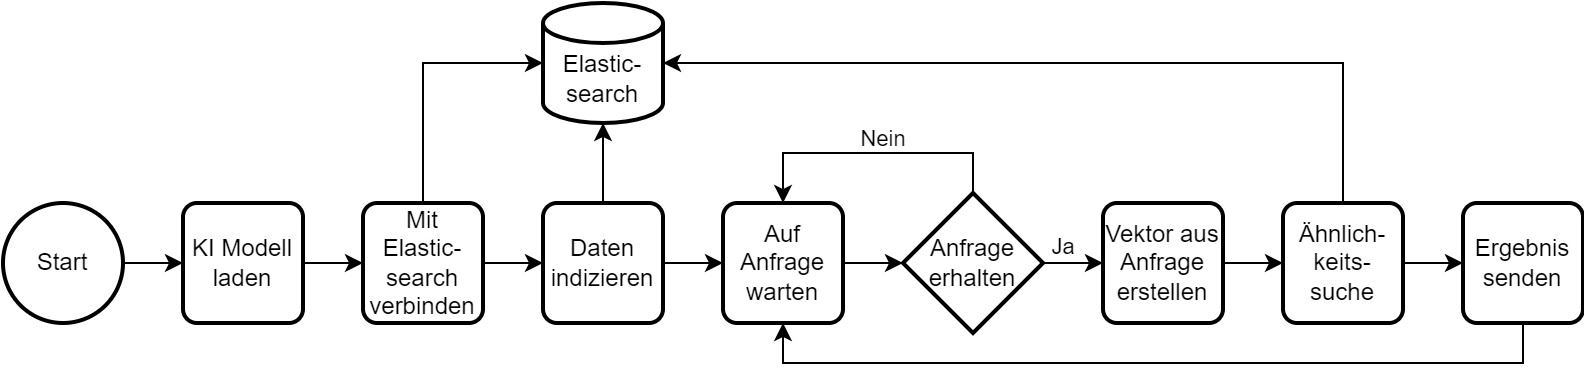
\includegraphics[width = 15cm]{bilder/KIAblauf}
    \caption{Ablaufdiagramm der Textähnlichkeitssuche}
\end{figure}

Damit der KI-Service eine Textähnlichkeitssuche durchführen kann, muss zunächst das BERT Modell importiert werden. Dieses kann der Service beim Starten automatisch aus dem offiziellen Tensorflow Hub herunterladen. Anschließen wird eine Tensorflow Session erstellt und gestartet. 

\begin{lstlisting}[language=Python]
embed = hub.Module("https://tfhub.dev/google/universal-sentence-encoder/2")
\end{lstlisting}

Im zweiten Schritt verbindet sich der Service mit der Elasticsearch Datenbank. Dazu wird die URL, unter der die Elasticsearch erreichbar ist aus den Environment Variablen geladen. Die Environment Variablen können entweder beim manuellen Starten des Services mitgegeben werden, oder falls der Service mit Docker gestartet wird, in der Docker-Compose File definiert werden. Mithilfe der URL initialisiert der Service eine Elasticsearch Instanz und speichert sie in der Variable \texttt{client} ab. 

\begin{lstlisting}[language=Python]
elasticsearch_url = os.environ.get('ELASTIC_URL')
client = Elasticsearch(elasticsearch_url)
\end{lstlisting}

Nachdem sich der Service erfolgreich mit der Elasticsearch verbunden hat, beginnt das Indizieren der Daten in der Datenbank. Dazu wird die Methode \texttt{index\_{}data()} aufgerufen. Der Datensatz, der für den Prototypen verwendet wurde, ist ein Auszug aus den gestellten Fragen im Forum Stackoverflow. In dem Datensatz sind 18.600 Fragen vorhanden. Jede Frage besteht aus einem Titel und einem Body. In einem Fragen-Body ist eine genauere Erläuterung der Frage, mit eventuellen Codeausschnitten oder Verlinkungen. Für die Indizierung ist lediglich der Titel der Frage genutzt worden. Das bedeutet im Umkehrschluss, dass der Titel der Frage repräsentativ für die gesamte Frage stehen muss. Nach Möglichkeit soll der Titel den gesamten Inhalt der Frage kurz und bündig zusammenfassen. Aus diesem Grund eignet  Stackoverflow sich besonders gut für den Datensatz, da in den Guidelines \glqq Write a title that summarizes the specific problem\grqq{} explizit erwähnt wird.\footcite{stackoverflow2022question}

Nach erfolgreicher Indizierung aller Fragestellungen, geht der Service in die Programmablaufschleife über. Die Schleife beginnt mit der Initialisierung der RabbitMQ Verbindung. Dort Verbindet sich der der Textähnlichkeitsservice mit der Queue \texttt{text-similarity}. Bei einer eingehenden Anfrage ruft die \texttt{callback} Funktion die \texttt{respond} Funktion auf, die den KI Algorithmus aufruft und sich um die Verarbeitung der Antwort kümmert. Die Funktion \texttt{handle\_{}query()} benötigt als Parameter die Query die vom Nutzer gestellt wurde und die Anzahl der Ergebnisse, die zurückgegeben werden sollen. Beide Parameter werden aus aus der Anfrage, die über RabbitMQ an den Service gesendet wurde, ausgelesen. Sollte es vorkommen, dass der Nutzer keine \texttt{search\_{}size} angegeben hat, wird der Standartwert 1 gesetzt.
 
\begin{lstlisting}[language=Python]
search_size = 1
    for p in params:
        if "search_size" in p.values():
            search_size = p["value"]

    message = handle_query(query, search_size)
\end{lstlisting}

Innerhalb der \texttt{handle\_{}query()} Methode wird zunächst der Satz, der vom Nutzer gesendet wurde, durch die Methode \texttt{embed\_{}text()} in einen Vektor konvertiert. Dieser  wird anschließend in das Feld \texttt{\glqq params\grqq{}} in der Such-Query für die Elasticsearch geschrieben. In dem Feld \texttt{\glqq source\grqq{}} wird die eigentliche Ähnlichkeitsanalyse definiert. Die Elasticsearch implementiert die Funktion \texttt{cosineSimilarity()}, die zwei Vektoren als Parameter annimmt. Der erste Vektor ist der  aus der Query zuvor generierte Vektor. Der zweite Vektor ist der aus dem Titel der Frage generierte Vektor. 

Mit der \texttt{client.search()} stellt der Service die Anfrage an die Elasticsearch mit der zuvor definierten Query. In der Anfrage wird über das Feld \texttt{\glqq size\grqq} die Anzahl der gewünschten Ergebnisse mitgeliefert. Wenn die \texttt{search\_{}size} beispielsweise 3 beträgt, werden die drei Fragen mit den ähnlichsten Vektoren in die Variable \texttt{response} geschrieben. Im nachfolgen Codesegment sind die zuvor beschriebene Erstellung des Query Vektors, der Such-Query für die Elasticsearch und die Anfrage an die Elasticsearch dargestellt.

\begin{lstlisting}[language=Python]
query_vector = embed_text([query])[0]
script_query = {
    [...]
        "source": "cosineSimilarity(params.query_vector, doc['title_vector']) + 1.0",
        "params": {"query_vector": query_vector}  
}
response = client.search(
    [...]
        body={
            "size": search_size,
            "query": script_query,
            [...]
        }
)
\end{lstlisting}

Die Response der Elasticsearch wird nach erfolgreicher Durchführung wieder an die \texttt{respond} Funktion übergeben. Dort wird die Nachricht vorbereitet, die als Response auf die Anfrage vom Backend zurückgesendet wird. Die Antwort wird an RabbitMQ in die Queue \texttt{response-text-similarity} gesendet.

Der Schleifendurchlauf des Services ist damit abgeschlossen. Der Service geht nun wieder, wie in Abbildung 7 zu sehen, zum Zustand \glqq Auf Anfrage warten\grqq{} über. 

\subsubsection{Management der Services}
Die entworfene Softwarearchitektur unterstützt eine beliebige Anzahl an KI-Services. Alle Services, die über das System erreichbar sein sollen, müssen über die API registriert werden. Jeder Service implementiert eine Verbindung zur RabbitMQ Schnittstelle, damit die Anfragen und Antworten asynchron zwischen dem Backend und dem jeweiligen Service gesendet werden können. Eine der Kernanforderungen für eine Architektur, die austauschbare KI-Services unterstützt, ist die dynamische Registrierung und Deregistrierung. Eine Registrierung beschreibt das Hinzufügen eines neuen Services im System, ohne den Quellcode anpassen zu müssen. Um dies zu ermöglichen, braucht es einen persistenten Speicher, in dem alle zur Verfügung stehenden Services aufgelistet sind. Zur persistenten Speicherung von kleineren Datenmengen, eignet sich eine MySQL Datenbank. Innerhalb der Datenbank werden alle aktiven Services in der Tabelle \texttt{services} abgespeichert. Zu jedem Service gibt es einen Namen, \texttt{servie}, und einen Anzeigenamen, \texttt{display\_{}name}. Der Name wird für das interne Routing über RabbitMQ genutzt. Der Anzeigename wird im Frontend innerhalb des Dropdowns für die Auswahl des Services verwendet.

\subsubsection{Automatisierte Transformation des Inputs}
Jeder Service
- KIs benötigen Daten in anderem Format
- Nicht benötigte Informationen vorhanden
- Keine Möglichkeit per Hand zu Filtern bei größeren oder live-daten
- JSON als Bauanleitung für das Transformieren
- Seperator um gleichzeitig mehrere Nachrichten an den KI service zu schicken
- Replace nutzt Regex um Textabschnitte zu ersetzen oder zu verändern
- Beliebige Anzahl an Replace Operationen -> im Array angegeben
- Beispiel-Json -> entfernt Zeitstempel der Form [12:25:10]

\begin{lstlisting}[language=Python]
{
  "seperator": "\n",
  "replace": [
    {
      "old":"\[(\d*:?)*\]",
      "new":""
    }
  ]
}
\end{lstlisting}

\subsubsection{Fehlerbehandlung}
Während des Laufzeit des Programms kann es dazu kommen, dass im vom Nutzer produzierte Fehler auftreten. Der Nutzer kann im Bereich der Transformation syntaktisch nicht korrekte Texte eingeben, die Backend verarbeitet werden. Da Nutzereingaben ohne weitere Behandlung ebenfalls ein Sicherheitsrisiko für die Infrastruktur darstellen können, wird im Backend ein System implementiert, um die Verarbeitung der Eingaben in einer isolierten Umgebung ausführen zu können. Ähnlich wie bei der Verifizierung des JWT, ist das System zur Fehlerbehandlung auch mit Function Wrappern und Annotations umgesetzt. 

Im Backend wird ein Exception Handler definiert der eine Funktion mit zuvor übergebenen Parametern ausführt. Da eine fehlerhafte Ausführung auch dort zum Programmabsturz führen würde, wird die Funktion in einem try-except Block gekapselt. Alle innerhalb dieses Blocks auftretende Fehler werden abgefangen und in einem Exception Objekt gespeichert. Innerhalb des Exception Objekts ist die produzierte Fehlermeldung gespeichert. Über \texttt{str(e)} kann auf die Fehlermeldung zugegriffen werden. Innerhalb des Except Blocks wird die Fehlermeldung an den Logger weitergegeben, um diese in einer Datenbank persistent zu speichern. Nach erfolgreichem Log wird dem Frontend in einer HTTP Response der Statuscode 500 \glqq Internal Server Error\grqq{} zurückgegeben.\footcite{fielding1999rfc2616}

\begin{lstlisting}[language=Python]
[...]
 @wraps(f)
        def decorator(*args, **kwargs):
            try:
                return f(*args, **kwargs)
            except Exception as e:
                logger.log("error", f"[Server, {msg}]: {str(e)}", "none")
                return r.respond({"success": False, "error": str(e)}, status=500)
            [...]
\end{lstlisting}

Jede Funktion, die in innerhalb des Exception Handlers ausgeführt werden soll, wird mit der Annotation \texttt{@exception\_{}handler("...")} versehen. Innerhalb des Parameters, wird der Ort, an dem die Funktion ausgeführt wird, und damit der Fehler auftritt, als String übergeben. Diese Information wird genutzt, um innerhalb des Fehlerlogs den Ort des Fehlers aufzulisten.

\subsubsection{Event Logging}
Das Backend implementiert ein Event Logging System mit dem Zustände und Informationen des Systems in einer Datenbank gespeichert werden können. Mithilfe von Logs können Entwickler den Ablauf eines Programms besser nachvollziehen und auftretende Fehler schneller zu ihrer Quelle zurückverfolgen. Es ist ebenfalls möglich, Systeme aufzusetzen, die die auf Logs auslesen und beim Auftreten eines Errors die zuständigen Personen alarmieren. Eine Herausforderung bei einem Logging System ist es, dass das System dem Entwickler beim Loggen keinen erheblichen Mehraufwand produzieren soll. Im Backend wurde ein Logging System entwickelt, welches mit einer einzigen Funktion angesteuert werden kann. Die Log Funktions des Loggers wird in den verschiedenen Bereichen der Anwendung über \texttt{from logs.logger import log} importiert. Nach erfolgreichem Import, steht die \texttt{log} Funktion zur Verfügung. 

Für einen Log müssen drei Parameter übergeben werden, der Log Level, eine Message und die UUID. Die möglichen Ausdrücke für die Log Level sind in Tabelle 2 aufgeführt. Die unterstützten Log Level leiten sich aus der Funktionalität von Grafana ab, welche diese Logs mit einer zugeordneten Farbe visualisiert.

\begin{table}[H]
\centering
\begin{tabular}{c|c|c}
\textbf{Ausdruck} & \textbf{Log Level} & \textbf{Farbe}\\
\hline
emerg & critical & lila\\
fatal & critical & lila\\
alert & critical & lila\\
crit & critical & lila\\
critical & critical & lila\\
err & error & rot\\
eror & error & rot\\
error & error & rot\\
warn & warning & gelb\\
warning & warning & gelb\\
info & info & grün\\
information & info & grün\\
notice & info & grün\\
dbug & debug & blau\\
debug & debug & blau\\
trace & trace & hellblau\\
* & unknown & grau
\end{tabular}
\caption{Log Level des Event Logging Systems}
\end{table}

Innerhalb der Log Funktion wird eine Datenbank Query mit den drei Parametern und einem aktuellen Zeitstempel erstellt. Der Zeitstempel kann mithilfe des \texttt{datetime} Packages erstellt werden. Über \texttt{cursor.execute()} wird die erstellte Query in der MySQL Datenbank ausgeführt. Der Log wird als Eintrag in der Tabelle \texttt{logs} gespeichert. 

\begin{lstlisting}[language=Python]
def log(level, message, uid):
    [...]
    query = f"INSERT INTO logs (`level`, `message`, `timestamp`, `uid`) VALUES (%s, %s, %s, %s)"
    cursor.execute(query, (level, message, datetime.utcnow(), str(uid)))
    [...]
\end{lstlisting}

\subsubsection{Website mit Angular}
text
\subsection{Deployment der Software mit Docker}
text